\documentclass[11pt]{article}

\usepackage[margin=1in]{geometry}
\usepackage{booktabs}
\usepackage{graphicx}
\usepackage{url}
\usepackage{hyperref}
\usepackage{amsmath}
\usepackage{float}

\title{Multi-Agent Reinforcement Learning in Pommerman: Comparing PPO and Dreamer-Style World Models}
\author{Kosta Karathanosopoulos \and Taari Chandaria \and Wilfred Allison \and Ryder Swenson}
\date{CS 1470 Final Project, Brown University, Spring 2026}

\begin{document}
\maketitle

\section{Introduction}

Many reinforcement learning methods are developed in settings where one agent acts in a mostly stationary environment. Multi-agent environments are harder: the world changes not only because of physics, but also because other agents make decisions. This makes learning especially difficult when rewards are sparse and delayed. A policy must learn what to do, while a model-based agent must also learn dynamics that include other agents' behavior.

We study this problem in Pommerman, a four-player grid-world inspired by Bomberman. Agents move through an $11 \times 11$ board, place bombs, destroy wooden walls, collect power-ups, and try to survive while eliminating opponents. Pommerman is small enough for a course-scale project, but it still requires spatial reasoning, safety, planning, and opponent awareness. This makes it a useful testbed for asking whether a learned world model can help in a competitive multi-agent environment.

Our project compares a model-free PPO baseline against Dreamer-style model-based agents. PPO learns directly from real rollouts using clipped policy-gradient updates. Dreamer instead learns a recurrent latent world model that predicts future board states, rewards, and episode continuation, then trains actor-critic policies through imagined rollouts. We implement three Dreamer variants: independent world models, a shared world model, and opponent-aware world models conditioned on other agents' recent actions and alive status.

The main result is nuanced. In the original 2048-step local study, PPO was the strongest early baseline, reaching an evaluation mean reward of $1.14$ and a $50\%$ win rate over a small evaluation set. Early Dreamer variants learned world-model signals but did not win. However, larger Oscar runs changed the story: PPO's final win rate stayed weak under stricter free-for-all (FFA) evaluation, while shared Dreamer variants achieved much stronger win rates. The strongest comparable FFA result was Shared Dreamer with imagination horizon $h=3$, which reached a final win rate of $43.75\%$ and a best logged win rate of $93.75\%$. We therefore conclude that PPO is a useful early sanity-check baseline, but shared world-model learning becomes promising with more compute and training support.

\section{Literature Review}

Our work builds on Dreamer, a model-based reinforcement learning agent introduced by Hafner et al. \cite{hafner2020dreamer}. Dreamer learns a recurrent state-space model (RSSM) from experience, uses it to imagine latent trajectories, and trains a policy and value function on those imagined rollouts. The original Dreamer setting is single-agent control, where the transition dynamics depend on the agent and a fixed environment.

Pommerman changes that assumption. In a single-agent model, the dynamics can be written as $p(s_{t+1} \mid s_t, a_t)$. In Pommerman, the next state depends on the joint action, closer to $p(s_{t+1} \mid s_t, a_t^1, a_t^2, a_t^3, a_t^4)$. If a world model ignores the other agents, it may produce misleading imagined futures. This is the central reason we test independent, shared, and opponent-aware Dreamer variants.

Pommerman was introduced by Resnick et al. as a multi-agent benchmark with FFA play, partial observability, communication variants, planning, and opponent modeling \cite{resnick2018pommerman}. The environment is also known to be difficult for standard RL because useful actions can be dangerous early in training. Bombs are necessary for winning, but weak agents often die from their own bombs, creating a passive local optimum.

PPO provides our model-free baseline \cite{schulman2017ppo}. PPO is relatively stable and simple, but it does not learn a dynamics model. In our experiments, PPO is useful as a baseline, but it also exposes an important metric issue: it trains on shaped rewards while we evaluate win rate using sparse terminal outcomes.

\section{Methodology}

\subsection{Environment and Observations}

Pommerman is a four-agent grid world with rigid walls, wooden walls, passage tiles, power-ups, bombs, flames, and agents. Each agent chooses one of six actions: Stop, Up, Down, Left, Right, or Bomb. We focus on four-player FFA Pommerman, where each agent competes to be the last survivor. The environment is hard because agents must avoid explosions, navigate obstacles, decide when to clear wood, collect power-ups, and reason about other agents' future positions.

We encode Pommerman's symbolic observations as tensors rather than rendered pixels. The board is represented with one-hot channels for tile types and agents. Additional feature planes encode bomb blast strength, bomb life, the controlled agent's position, ammo, blast strength, and kick ability. This keeps the problem spatial while avoiding the cost of visual perception from raw frames.

\subsection{Models}

The PPO baseline uses a convolutional encoder followed by actor and critic heads. The actor outputs a categorical distribution over six actions, and the critic predicts state value. PPO is trained from real trajectories using generalized advantage estimation with $\gamma=0.99$ and $\lambda=0.95$, a clipped objective with ratio $0.2$, entropy regularization, and multiple minibatch epochs.

The Dreamer agents use a recurrent latent world model. Observations pass through a CNN encoder. A GRU-based RSSM maintains a deterministic state and a stochastic latent state. The world model predicts rewards, continuation, board reconstruction, and scalar observation features. The actor and critic operate on latent features and are trained from imagined rollouts. In the Oscar experiments, the main Dreamer runs used latent dimension 64, hidden dimension 256, sequence length 16, batch size 24, replay buffers between 16k and 32k, and imagination horizons 1, 3, or 5.

Action masking means explicitly marking invalid actions as unavailable before sampling or training the policy, so agents do not waste updates on impossible or useless actions such as walking into walls or placing a bomb with no ammo. This was especially important for Dreamer, because imagined rollouts can otherwise let the actor exploit unrealistic actions inside an imperfect model.

\paragraph{Independent Dreamer.}
Each controlled agent has its own world model, actor, and critic. This allows specialization, but every agent must learn similar board physics separately.

\paragraph{Shared Dreamer.}
Agents share one world model while keeping separate actor and critic heads. This assumes that Pommerman's physical rules are common across agents. Our Oscar results support this design: shared horizon-3 and horizon-5 were the strongest comparable FFA Dreamer runs.

\paragraph{Opponent-Aware Dreamer.}
Each agent conditions its model on other agents' recent actions and alive status. This directly addresses multi-agent non-stationarity, but it also makes the model harder to optimize. In our runs, opponent-aware models sometimes reached very high best win rates but were less stable than the best shared model.

\section{Challenges}

The hardest part of the project was making the whole multi-agent RL pipeline trustworthy enough to interpret. Pommerman forced us to handle environment wrapping, observation encoding, reward shaping, recurrent replay, action validity, checkpointing, logging, evaluation, and visualization.

The first challenge was reward design. Sparse terminal rewards provide little feedback, and bombs create a bad local optimum: early bomb use often kills weak agents, so agents can learn to survive passively instead of learning to win. We therefore used shaped rewards that preserved win/loss signals while adding intermediate terms for destroying wood, collecting power-ups, eliminating enemies, useful bombs, wasted bombs, blocked moves, ties, and step costs.

This shaped reward helped training, but it also complicated interpretation. PPO can improve dense shaped reward without reliably winning games. This explains why PPO Long achieved a better best reward than short PPO but ended with only a $6.25\%$ final win rate. For this reason, we report final reward, best reward, final win rate, and best win rate separately.

The second challenge was Dreamer's recurrent replay. The RSSM needs valid same-episode sequences; sampling across episode boundaries would corrupt the hidden state. We added sequence-aware replay checks to avoid training on invalid recurrent trajectories.

The third challenge was the gap between world-model learning and control. In the early local runs, Dreamer world-model losses decreased, but the policies still did not win. This taught us to distinguish ``the model predicts something'' from ``the actor can use the model for good decisions.'' The larger Oscar runs show that this gap can shrink, especially for shared Dreamer, but it remains the key difficulty.

Finally, evaluation itself was noisy. Pommerman wins are sparse, and many evaluations used small episode batches. Several methods spiked and then collapsed. Reporting both best and final win rate is therefore important: best win rate shows whether a method ever found a strong policy, while final win rate shows whether training preserved it.

\section{Results}

We report three pieces of evidence: the original short local study, later local/debugging runs that achieved nonzero Dreamer performance, and the larger Oscar FFA matrix.

\subsection{Local and Debugging Runs}

The first 2048-step local study validated that the pipeline worked, but it was too small to settle the algorithm comparison. PPO won early, while the initial Dreamer variants learned world-model signals but got zero wins. Later local debugging and optimized shared-Dreamer runs produced nonzero model-based performance, including a best-checkpoint evaluation of approximately $17.2\%$ win rate over 64 episodes.

\begin{table}[H]
\centering
\resizebox{\linewidth}{!}{
\begin{tabular}{lrrrr}
\toprule
Run & Steps & Final reward & Best reward & Best win rate \\
\midrule
PPO baseline & 2048 & 1.140 & 1.140 & 50.0\% \\
Independent Dreamer & 2048 & -1.000 & -0.830 & 0.0\% \\
Shared Dreamer & 2048 & -1.000 & -0.958 & 0.0\% \\
Opponent-aware Dreamer & 2048 & -1.000 & -0.675 & 0.0\% \\
Optimized Shared Dreamer ($h=1$) & 32768 & -- & -- & 17.2\% \\
\bottomrule
\end{tabular}
}
\caption{Local and debugging-stage results. The original 2048-step study favored PPO, but later optimized shared-Dreamer runs showed nonzero model-based control before the full Oscar matrix.}
\label{tab:local-results}
\end{table}

\subsection{Oscar FFA Results}

Table \ref{tab:oscar-results} shows the final Oscar FFA results. The main shift is that PPO no longer dominates. Short PPO finished with $0\%$ final win rate, and PPO Long finished with only $6.25\%$ final win rate despite reaching $31.25\%$ best win rate. Shared Dreamer $h=3$ was the strongest comparable final result, ending at $43.75\%$ win rate and reaching $93.75\%$ at its best checkpoint.

\begin{table}[H]
\centering
\resizebox{\linewidth}{!}{
\begin{tabular}{lrrrrrr}
\toprule
Experiment & Final reward & Best reward & Final win rate & Best win rate & Eval points & Last step \\
\midrule
PPO & -1.363 & -1.363 & 0.0\% & 6.25\% & 16 & 32768 \\
PPO Long & -0.228 & 0.569 & 6.25\% & 31.25\% & 64 & 262144 \\
Independent Dreamer ($h=3$) & -0.631 & -0.584 & 0.0\% & 81.25\% & 11 & 24216 \\
Shared Dreamer ($h=1$) & -0.602 & -0.592 & 0.0\% & 18.75\% & 12 & 25952 \\
Shared Dreamer ($h=3$) & -0.361 & -0.225 & 43.75\% & 93.75\% & 12 & 24856 \\
Shared Dreamer ($h=5$) & -0.456 & -0.209 & 31.25\% & 68.75\% & 11 & 23156 \\
Opponent-aware Dreamer ($h=3$) & -2.433 & -0.062 & 0.0\% & 100.0\% & 16 & 32768 \\
Opponent-aware stable ($h=3$) & -0.988 & 0.001 & 37.5\% & 100.0\% & 64 & 131072 \\
\bottomrule
\end{tabular}
}
\caption{Oscar FFA results. Shared Dreamer with horizon 3 was the strongest comparable final result. PPO improved somewhat with longer training, but had low final win rate under the sparse terminal-win metric.}
\label{tab:oscar-results}
\end{table}

The shared Dreamer results are the strongest positive finding. They suggest that Pommerman contains common physical dynamics that can be learned more efficiently by a shared model than by separate independent models. The horizon ablation is also informative: horizon 1 was too short, horizon 3 performed best, and horizon 5 remained strong but slightly weaker. This matches the intuition that Pommerman requires planning over delayed bomb effects, but long imagination can amplify model error.

The opponent-aware results were high variance. Both opponent-aware variants reached $100\%$ best logged win rate, but the non-stabilized run collapsed to $0\%$ final win rate, and the stabilized version ended below Shared Dreamer $h=3$. Opponent conditioning is therefore promising, but harder to optimize than simple sharing.

\begin{figure}[H]
\centering
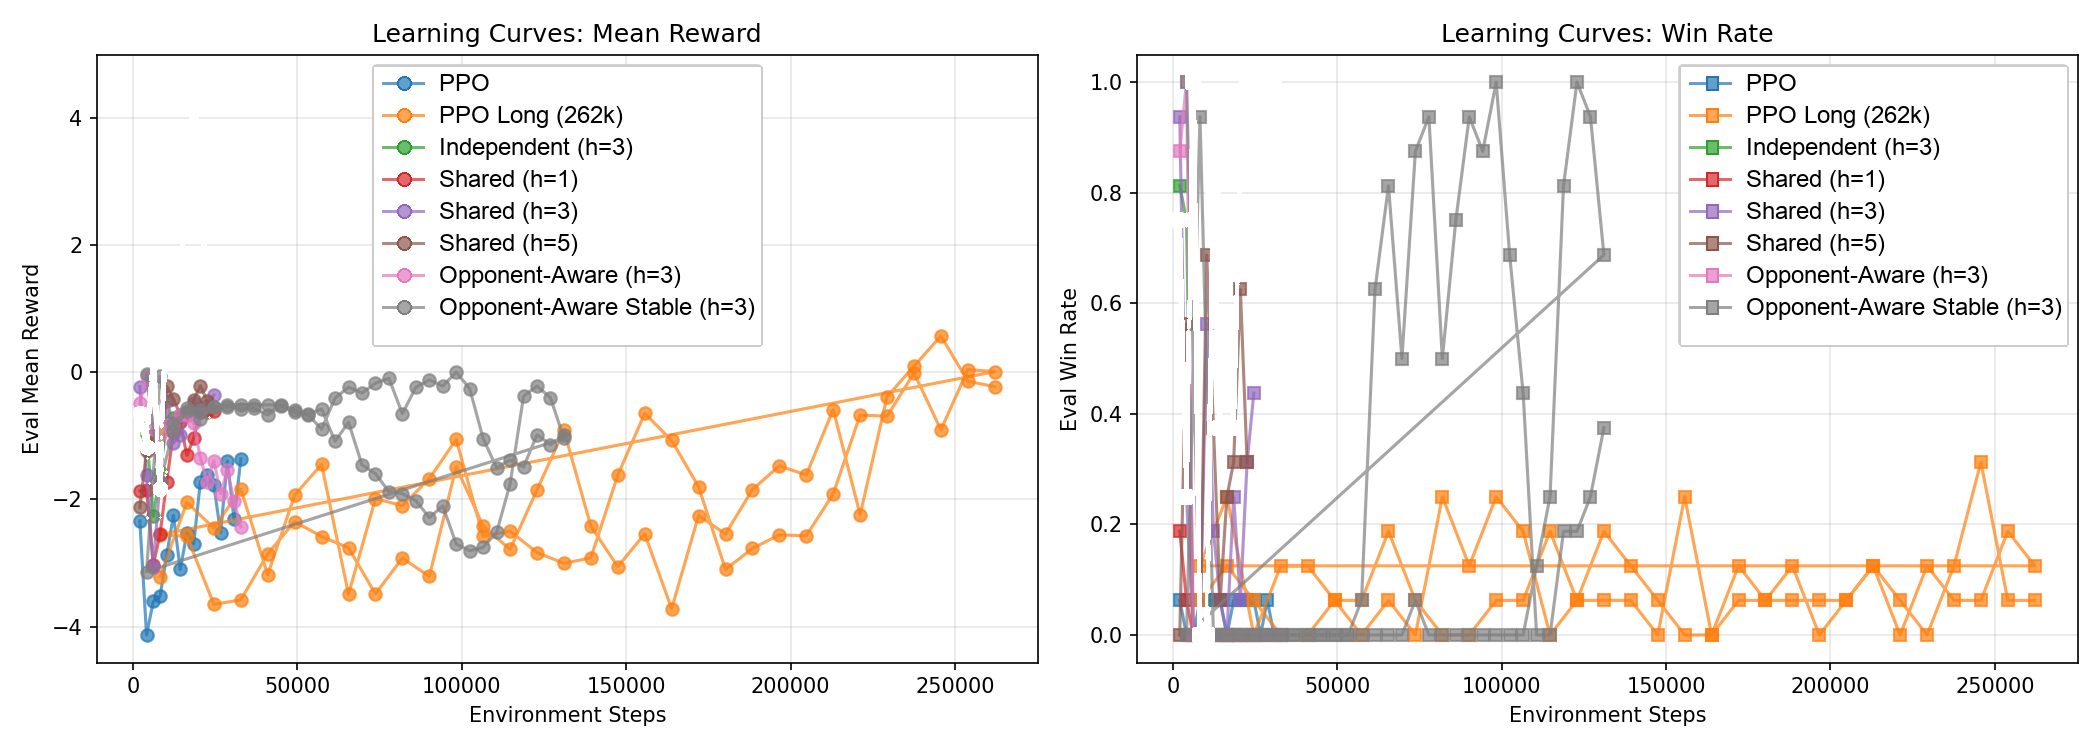
\includegraphics[width=\linewidth]{results/final_results.png}
\caption{Oscar reward and win-rate curves. Win rate is noisy, but Shared Dreamer $h=3$ and stabilized opponent-aware Dreamer achieve much stronger FFA win rates than PPO at their best checkpoints.}
\label{fig:curves}
\end{figure}

Overall, the results support four conclusions. First, PPO is useful for early validation but does not reliably optimize terminal wins in our Oscar FFA runs. Second, shared world-model learning is the strongest Dreamer adaptation we tested. Third, opponent-aware modeling can produce strong peaks but was less stable. Fourth, reward shaping, action masking, checkpoint selection, and evaluation variance are central to interpreting multi-agent RL results in Pommerman.

\section{Ethics}

This project uses a benchmark game environment and does not involve personal data, human subjects, private information, or real-world deployment. The direct ethical risks are limited, but multi-agent RL methods can eventually transfer to higher-stakes domains such as robotics, markets, cybersecurity, or autonomous decision-making. Agents trained only to optimize reward can learn unwanted adversarial behavior, so benchmark results should not be presented as deployment-ready systems.

There are also compute and reward-design considerations. Larger model-based experiments require more energy, so claims about sample efficiency should account for total training cost. Reward shaping also encodes design choices. We penalized passive behavior and wasted bombs to avoid local optima, but shaped reward is not the same as solving the original sparse benchmark. For that reason, we report shaped reward and terminal win rate separately.

\section{Reflection and Future Work}

The main lesson we learned is that model-based RL is not just about learning a predictive model. It is about learning a predictive model that is useful for control. A world model can reconstruct board states and reduce loss while still missing rare but important events, such as whether a bomb traps the agent or whether an opponent can escape.

We also learned that multi-agent RL magnifies every engineering problem. In Pommerman, failure can come from the environment wrapper, observation encoding, invalid actions, sparse rewards, recurrent replay, opponent behavior, world-model error, actor-critic instability, or evaluation noise. The tests, JSONL logs, checkpointing, reward diagnostics, and visualizations were necessary for understanding which failure we were seeing.

The results changed how we think about both PPO and Dreamer. PPO looked strongest in the tiny local study, but the Oscar runs revealed a gap between shaped-reward optimization and terminal wins. Dreamer initially looked mostly negative, but larger shared-model runs showed that model-based control can become competitive once the world model has enough capacity, replay, warmup, action masking, and compute.

Future work should first run more seeds and larger evaluation batches, since our win-rate estimates are noisy. Second, it should use better checkpoint selection: several runs found strong policies and then lost them by the final checkpoint. Third, PPO should be strengthened with consistent action masking, tuned entropy and learning-rate schedules, and rewards more closely aligned with terminal wins. Fourth, opponent modeling should be improved beyond recent actions and alive status, possibly with policy-belief models or centralized critics. Finally, a curriculum over simpler boards, fewer agents, or subgoals such as safe navigation and wood destruction could make Dreamer training more stable.

In the end, our project produced a more nuanced result than we expected. PPO was strongest in the tiny local study, but Shared Dreamer $h=3$ became the strongest comparable method in the larger Oscar FFA runs. This shows both sides of the model-based RL tradeoff: Dreamer-style methods are harder to train, but with shared dynamics, short-horizon imagination, shaped rewards, action masking, and enough compute, they can outperform the PPO baseline on terminal win rate.

\begin{thebibliography}{9}

\bibitem{resnick2018pommerman}
Cinjon Resnick, Wes Eldridge, David Ha, Denny Britz, Jakob Foerster, Julian Togelius, Kyunghyun Cho, and Joan Bruna.
\newblock Pommerman: A Multi-Agent Playground.
\newblock \emph{AIIDE Workshops}, 2018.
\newblock \url{https://arxiv.org/abs/1809.07124}

\bibitem{hafner2020dreamer}
Danijar Hafner, Timothy Lillicrap, Jimmy Ba, and Mohammad Norouzi.
\newblock Dream to Control: Learning Behaviors by Latent Imagination.
\newblock \emph{International Conference on Learning Representations}, 2020.
\newblock \url{https://arxiv.org/abs/1912.01603}

\bibitem{schulman2017ppo}
John Schulman, Filip Wolski, Prafulla Dhariwal, Alec Radford, and Oleg Klimov.
\newblock Proximal Policy Optimization Algorithms.
\newblock arXiv:1707.06347, 2017.
\newblock \url{https://arxiv.org/abs/1707.06347}

\bibitem{ng1999reward}
Andrew Y. Ng, Daishi Harada, and Stuart Russell.
\newblock Policy Invariance Under Reward Transformations: Theory and Application to Reward Shaping.
\newblock \emph{International Conference on Machine Learning}, 1999.

\bibitem{assran2023ijepa}
Mahmoud Assran, Quentin Duval, Ishan Misra, Piotr Bojanowski, Pascal Vincent, Michael Rabbat, Yann LeCun, and Nicolas Ballas.
\newblock Self-Supervised Learning from Images with a Joint-Embedding Predictive Architecture.
\newblock \emph{CVPR}, 2023.
\newblock \url{https://arxiv.org/abs/2301.08243}

\bibitem{maes2026leworldmodel}
Lucas Maes, Quentin Le Lidec, Damien Scieur, Yann LeCun, and Randall Balestriero.
\newblock LeWorldModel: Stable End-to-End Joint-Embedding Predictive Architecture from Pixels.
\newblock arXiv:2603.19312, 2026.
\newblock \url{https://arxiv.org/abs/2603.19312}

\end{thebibliography}

\end{document}
